% Reciprocal BLAST
%
% Simple introduction to reciprocal best BLAST matches

\subsection{Reciprocal BLAST}
\begin{frame}
  \frametitle{Reciprocal Best BLAST Hits (RBBH)}
  \begin{itemize}
    \item To compare our genecall proteins to \texttt{NC\_004547.faa} reference set...
    \item BLAST reference proteins against our proteins
    \item BLAST our proteins against reference proteins
    \item Pairs with each other as best BLAST Hit are called RBBH
  \end{itemize}
\end{frame}

\begin{frame}
  \frametitle{One-way BLAST vs RBBH}   
  One-way BLAST includes many low-quality hits \\
  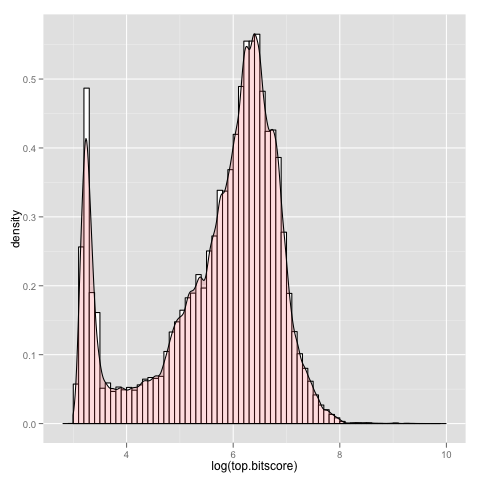
\includegraphics[width=0.3\textwidth]{images/rbbh1}
  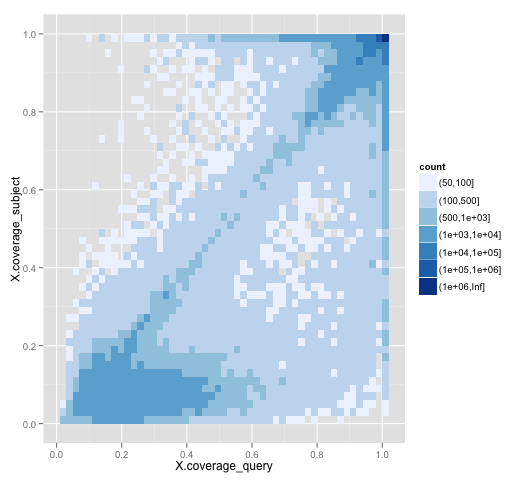
\includegraphics[width=0.33\textwidth]{images/rbbh2}
  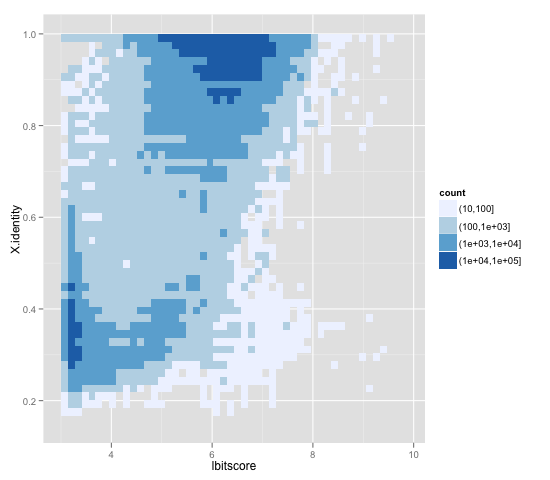
\includegraphics[width=0.34\textwidth]{images/rbbh3}
\end{frame}

\begin{frame}
  \frametitle{One-way BLAST vs RBBH}   
  Reciprocal best BLAST hits remove many low-quality matches \\
  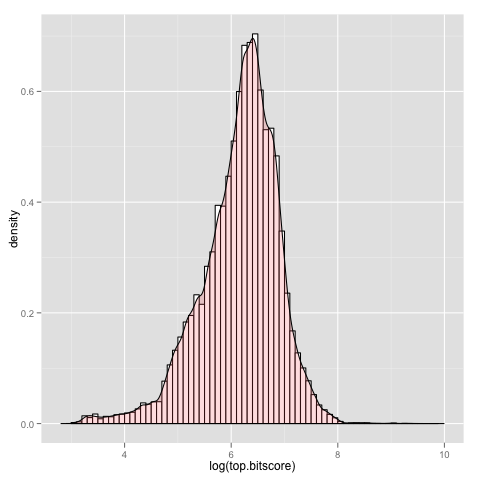
\includegraphics[width=0.3\textwidth]{images/rbbh4}
  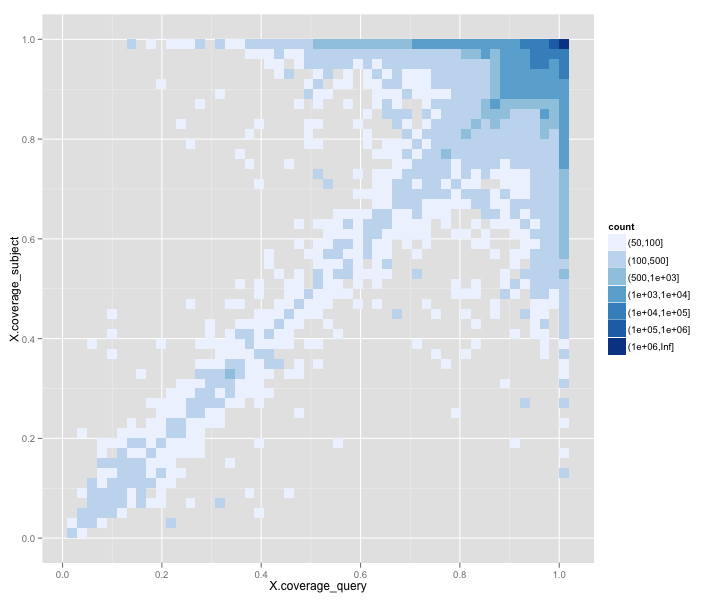
\includegraphics[width=0.34\textwidth]{images/rbbh5}
  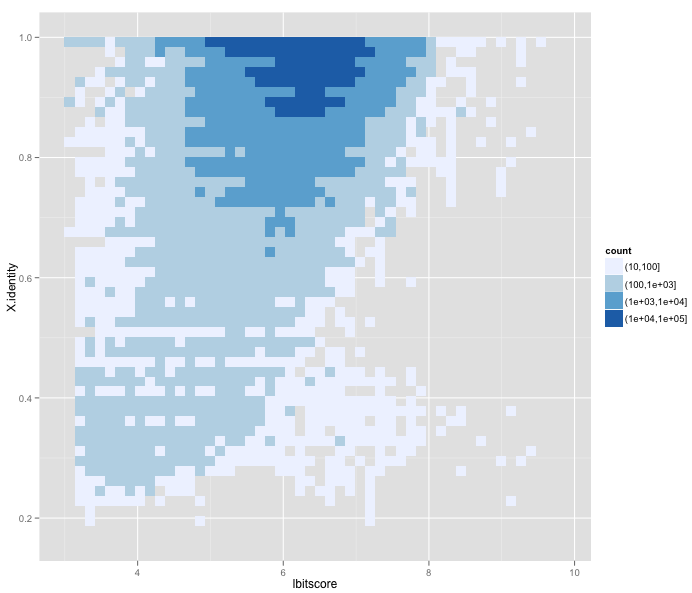
\includegraphics[width=0.34\textwidth]{images/rbbh6}
\end{frame}

\begin{frame}
  \frametitle{Reciprocal Best BLAST Hits (RBBH)}
  \begin{itemize}
    \item Pairs with each other as best BLAST hit are called RBBH
    \item Should filter on percentage identity and alignment length
    \item RBBH pairs are candidate orthologues
    \begin{itemize}
      \item (most orthologues will be RBBH, but the relationship is complicated)
      \item Outperforms OrthoMCL, etc. (beyond scope of course why and how$\ldots$) \\
           \url{http://dx.doi.org/10.1093/gbe/evs100} \\
           \url{http://dx.doi.org/10.1371/journal.pone.0018755}
    \end{itemize}
  \end{itemize}
  (We have a tool for this on our in-house Galaxy server)
\end{frame}

% Test data generated locally using FASTA protein files made with Artemis,
% and the underlying Python script for my Galaxy BLAST RBH tool available
% from https://github.com/peterjc/galaxy_blast/tree/master/tools/blast_rbh
% Here I *DID NOT* import minimum coverage or identity thresholds!
%
% /mnt/galaxy/galaxy_blast/tools/blast_rbh/blast_rbh.py NC_004547.faa chrA_prodigal.fasta -o rbbh_ref_vs_chrA_prodigal.tab -t blastp -a prot
% /mnt/galaxy/galaxy_blast/tools/blast_rbh/blast_rbh.py NC_004547.faa chrB_prodigal.fasta -o rbbh_ref_vs_chrB_prodigal.tab -t blastp -a prot
% /mnt/galaxy/galaxy_blast/tools/blast_rbh/blast_rbh.py NC_004547.faa chrC_prodigal.fasta -o rbbh_ref_vs_chrC_prodigal.tab -t blastp -a prot
% /mnt/galaxy/galaxy_blast/tools/blast_rbh/blast_rbh.py NC_004547.faa chrD_prodigal.fasta -o rbbh_ref_vs_chrD_prodigal.tab -t blastp -a prot